
After the discovery of the new boson, the next most important topic is to examine its properties. 
The SM Higgs is predicted to have $J^{CP} = 0^{++}$ where J is the spin, C is the charge, 
and P is the parity. In some BSM models such as SUSY, 
the Higgs sector can be expanded to CP-odd scalar or psedoscalar particles, 
or a mixture of them that leads to CP-violation.
Spin-1 model is excluded because the new boson decays to two massless bosons, 
\textit{i.e.}, photons, which is not possible for a massive spin-1 resonance 
due to Yang's theorem~\cite{PhysRev.77.242}. 
So, we intend to study alternative spin-0 and spin-2 models.   


In the reference~\cite{Bolognesi:2012mm}, phenomenological studies of the scattering 
amplitudes of SM Higgs or exotic boson wth different spin-parity natures are performed.  
The study shows that \hww\ channel has a good 
sensitivity to distinguish the SM Higgs from a graviton-like spin-2 resonance that couples to 
the \ww\ through a minial couplings. In this chapter this model is denoted as $2_{min}^+$
and the SM Higgs boson is denoted as $0^+$. We also test the pseudo-scalar spin-0 
boson which is denoted as $0^-$.

This section descirbes the spin-2 model, the helicity argument 
of \ww\ decay, method of study and the result. 

%%%%%%%%
\section{Models} 

A general form of the scattering amplitude of a spin-zero resonance that decays 
to two vector bosons is~\cite{Bolognesi:2012mm} 
\begin{eqnarray} 
A(X \rightarrow V_1V_2)
&=& 
\frac{1}{v^2} \epsilon^{\mu*}_1 \epsilon^{\nu*}_2 
\left( a_1 g_{\mu\nu}\mHi^2 + a_2q_\mu q_\nu 
     + a_3 \epsilon_{\mu\nu\alpha\beta} q_1^\alpha q_2^\beta \right)
\end{eqnarray} 
In this parametrization, the SM Higgs has $a_1 \neq 0$ and $a_2=a_3=0$, 
and the spin-0 pseudo-scalar boson has $a_3 \neq 0$ and $a_1=a_2=0$.
The helicity amplitudes are combination of $A_{00}$, $A_{++}$ and $A_{--}$ 
in case of SM Higgs boson, and $A_{++}$ and $A_{--}$ for the spin-0 
pseudo-scalar boson where $A_{00}$ is both Ws are longitudinally polarized, 
$A_{++}$ is when both Ws are helicity +1, and $A_{--}$ is when both Ws are helicity -1.  

A general form of scattering amplitude of a spin-two resonance that decays to two vector 
bosons is given in~\cite{Bolognesi:2012mm}. The minimal coupling scenario 
where only two couplings are non-zero gives the scattering amplitude 
\begin{eqnarray} 
A(X \rightarrow V_1V_2)
&=& 
\frac{1}{\Lambda^2}  
\left[ 
2 g_2^{(2)} t_{\mu\nu} \frac{q_\alpha q_\beta}{\Lambda^2} 
f^{(1)\mu\alpha*} f^{(2)\nu\beta*} 
+ 
2 m_V^2 g_5^{(2)} t_{\mu\nu} 
\epsilon^{\mu*}_1 \epsilon^{\nu*}_2 
\right] 
\end{eqnarray} 
where $\Lambda$ is the energy scale where new physics occur, 
$g_2^{(2),(5)}$ are the couplings, 
$t_{\mu\nu}$ is the wave function of X given by a symmetric traceless tensor, 
$q_{\alpha}$ is the 4-momentum of X, 
$f^{(i)\mu\alpha}$ is the field strength tensor given by 
    $\epsilon_i^\mu q_i^\alpha - \epsilon_i^\alpha q_i^\mu$, 
$m_V$ is the mass of gauge boson, and 
$\epsilon_i^{\mu}$ is the polarization vector of the gauge boson i.
This is the model similar to the spin-2 graviton with minimal couplings~\cite{Bolognesi:2012mm}. 
Apart from the spin-0 case, the spin-2 amplitude is a combination of 
all possible helicity amplitudes, so it is not easy to isolate the 
amplitude to specific helicity amplitudes. 

Because of the difference in the spin structure of $0^+$, $0^-$ and $2_{min}^+$ models, 
the angular distributions of the decaying particles in these models are different.  
Figure~\ref{fig:spinpaper} shows the azimuthal angle difference($\Phi$) between 
two leptons at the generator level. It shows that the angular distribution is 
different between models. 

%Because of different spin structure of SM Higgs boson and the $2_{min}^+$ model, 
%the kinematics of the two bosons that decay from the resonance is different. 
%A simple argument can be given based on the helicity conservation. 
%This can be expressed using Wigner's d-matrix~\cite{}, $D^{j}_{m'm}$, where 
%j is the total spin of the system, and  m' and m are the z-component of spin 
%in the initial resonance and the final boson system. 
%Let's assume that the beam axis is long the z axis and consider 
%decay of gauge bosons in the rest frame of SM Higgs boson. 
%The decay plane(the line that the two bosons are in when they fly away each other) 
%of the two bosons do not have any preference because SM Higgs boson has spin-0. 
%The Wigner's d-matrix in this case is $D_{00}^{0} = 1$. 
%On the other hand, in case of the $2_{min}^+$ model, in order for the 
%total helicity to be 0 in the boson system, the bosons   
%\textcolor{red}{how to proceed for spin-2 case? Is $2_{min}^+$ in $|2,2>$ state?
%then, d-function is $\left( \frac{1+\cos \theta}{2} \right)^2$ and this is 
%consistent with blue tri-angle in the Phi plot in the middle.} 


\begin{figure}[htp] 
\centering 
\begin{tabular}{c} 
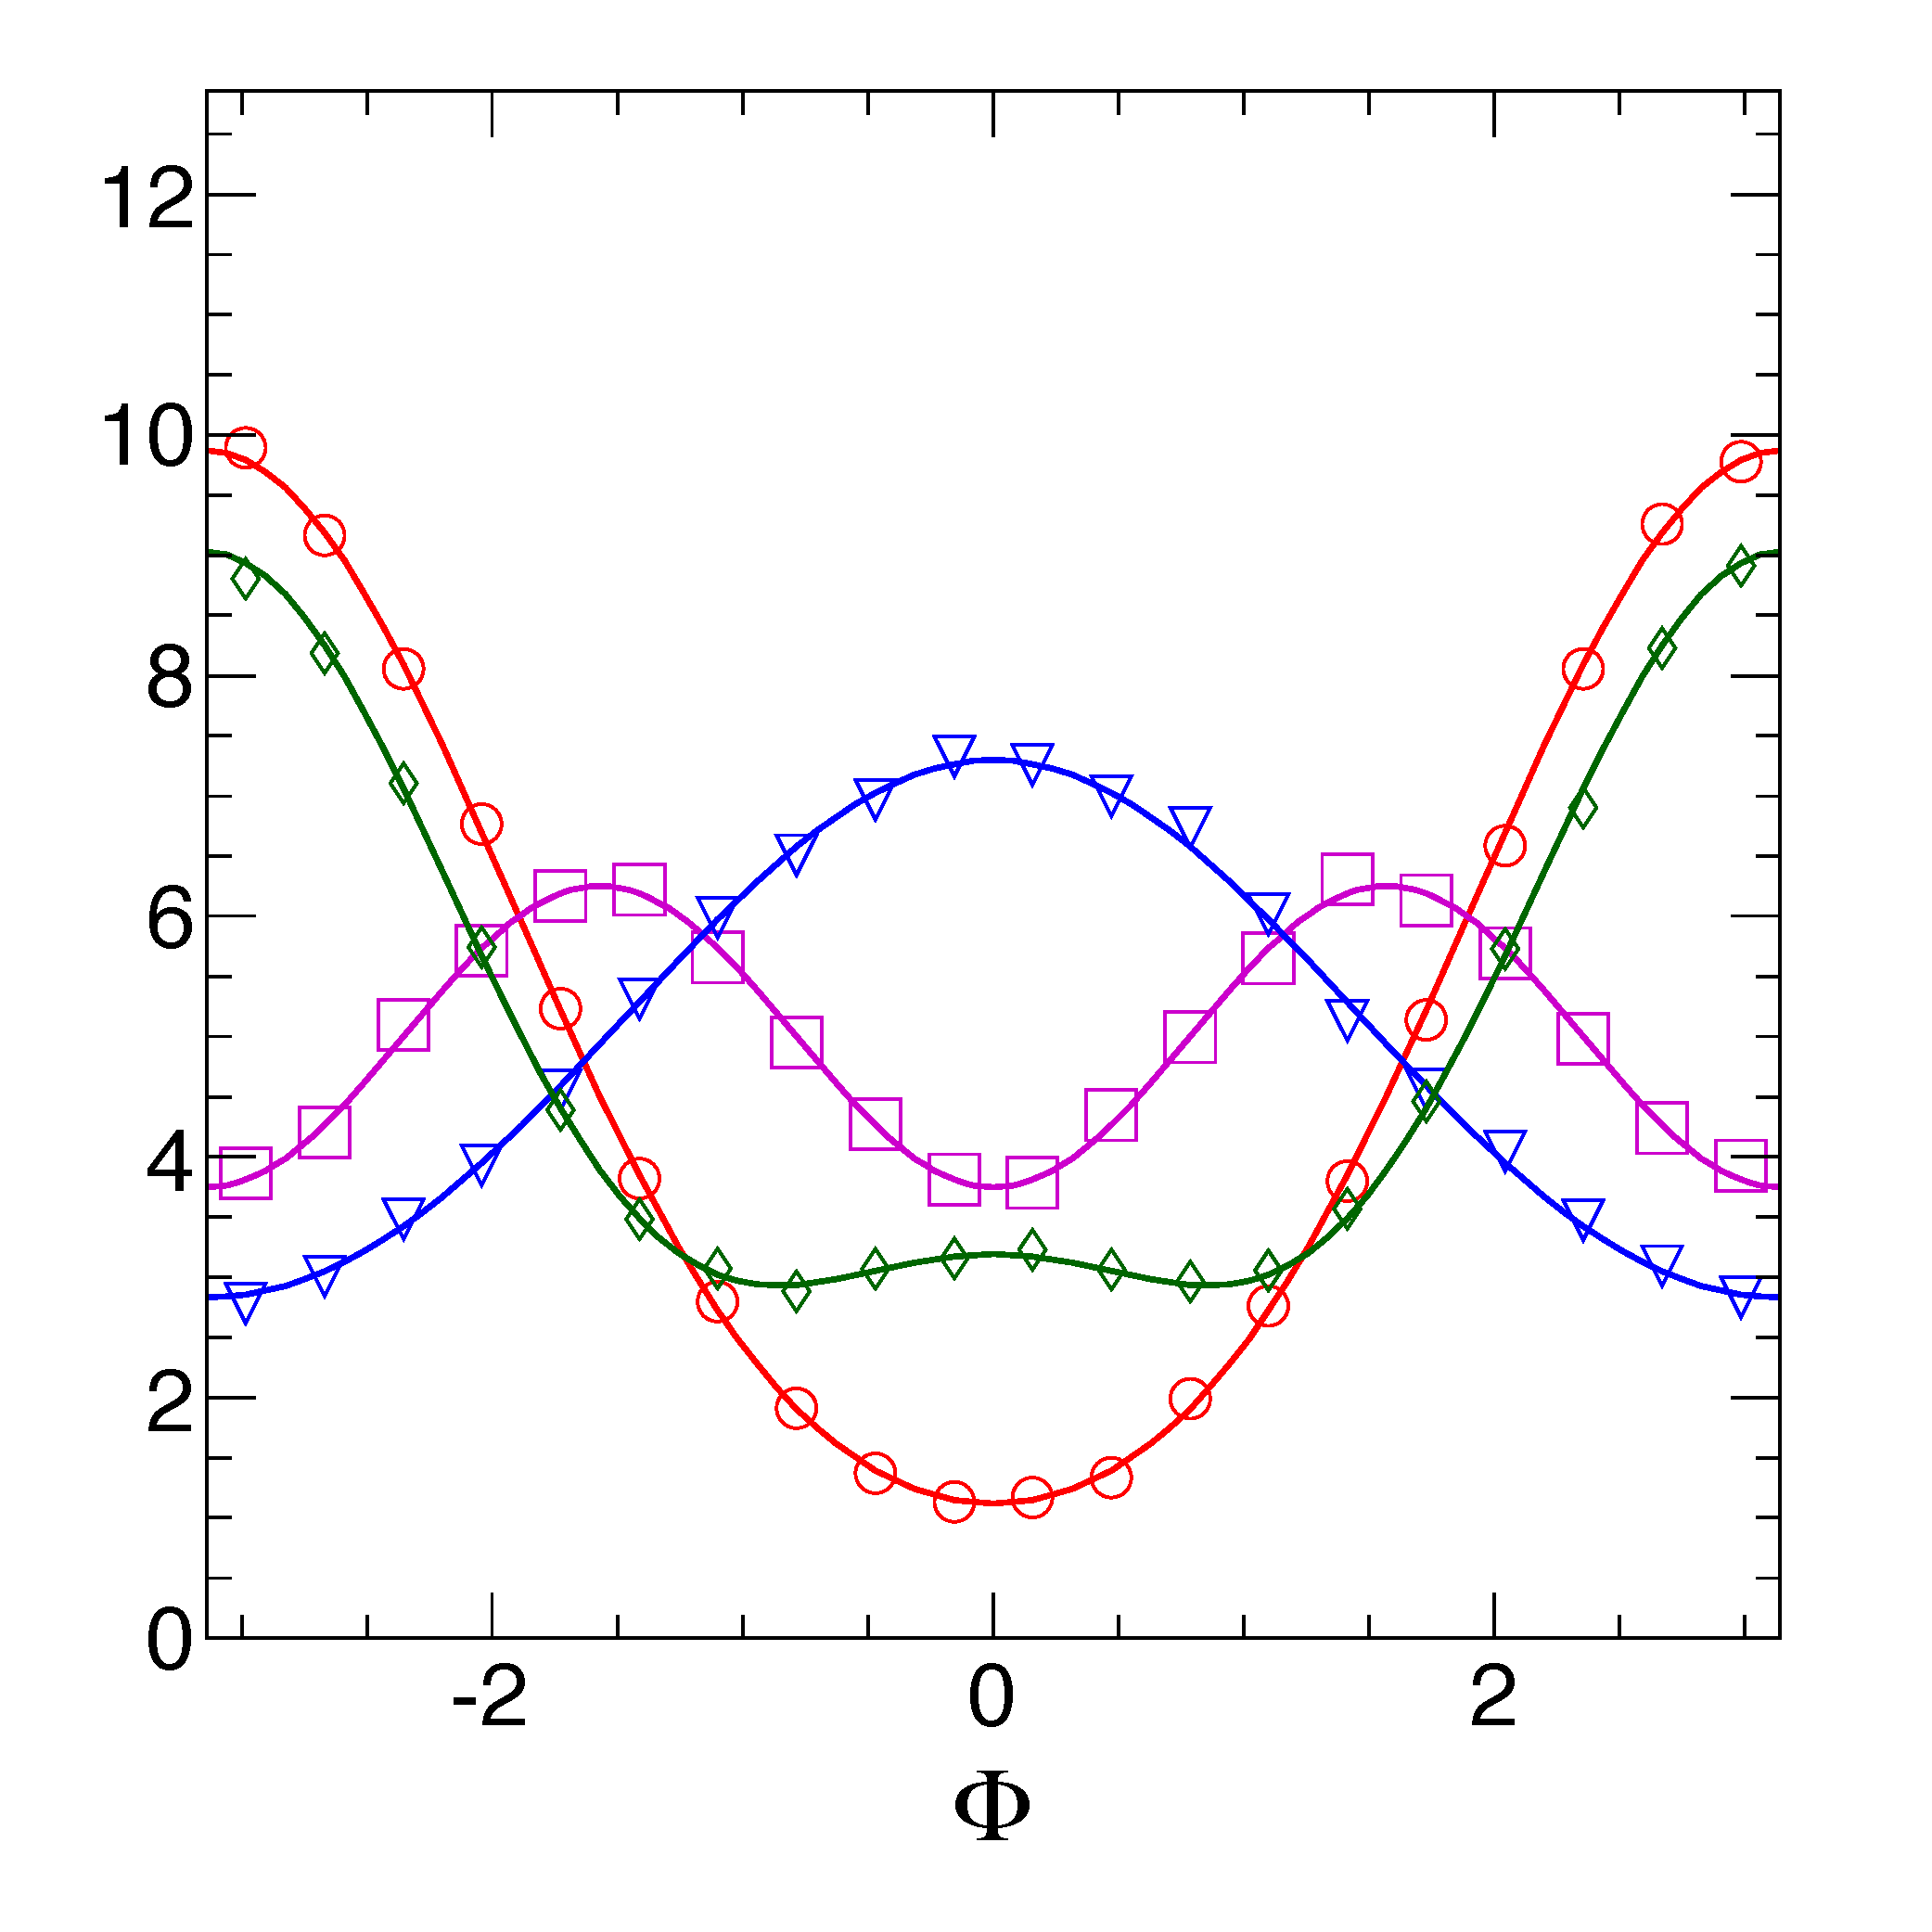
\includegraphics[width=0.5\textwidth]{figures/SpinPaper.pdf} 
\end{tabular} 
\caption{The azimuthal angle difference($\Phi$) between
two leptons at the generator level. The red circle is the SM Higgs boson($0^+$),
the magenta square is the $0^-$ model, and the blue triangle is the $2_{min}^+$ model.} 
\label{fig:spinpaper} 
\end{figure} 

The spin-2 sample is generated by the JHUGen~\cite{Bolognesi:2012mm,Gao:2010qx} generator 
with the matrix element calculation at a leading-order(LO). 
The rest of the simulation for parton showering, hadronization, and underlying events 
is done by PYTHIA~\cite{Sjostrand:2006za}. The JHUGen generator is validated 
by generating the SM Higgs boson events, and comparing it with the result 
of MCFM~\cite{Campbell:2010ff}. 
At the reconstruction level, JHUGen+PYTHA is validated by comparing kinematic 
distributions with the result of POWHEG+PYTIHA.
Both comparisons show good agreement~\cite{GaoAN}. 

%%%%%%%%
\section{Test Method}

\subsubsection{Templates}

In order to distinguish between the SM Higgs boson and an alternate model,
we first construct the 2-dimensional templates with \mT\ and \mll\ for the signal 
and the background processes in \DF\ 0-jet and 1-jet categories..
We use the same 2-dimensional templates 
as used for the SM Higgs search, which are described in detail in 
section~\ref{sec:shape}. At the generator level, 
\delphill\ is the best variable that separates the two hypotheses. 
But, after selections are applied to suppress backgrounds, and the boost of Higgs system 
is taken into account, the separation power is diluted, and \mll\ gives a better 
separation power. 

\begin{figure}[ht!] 
\centering 
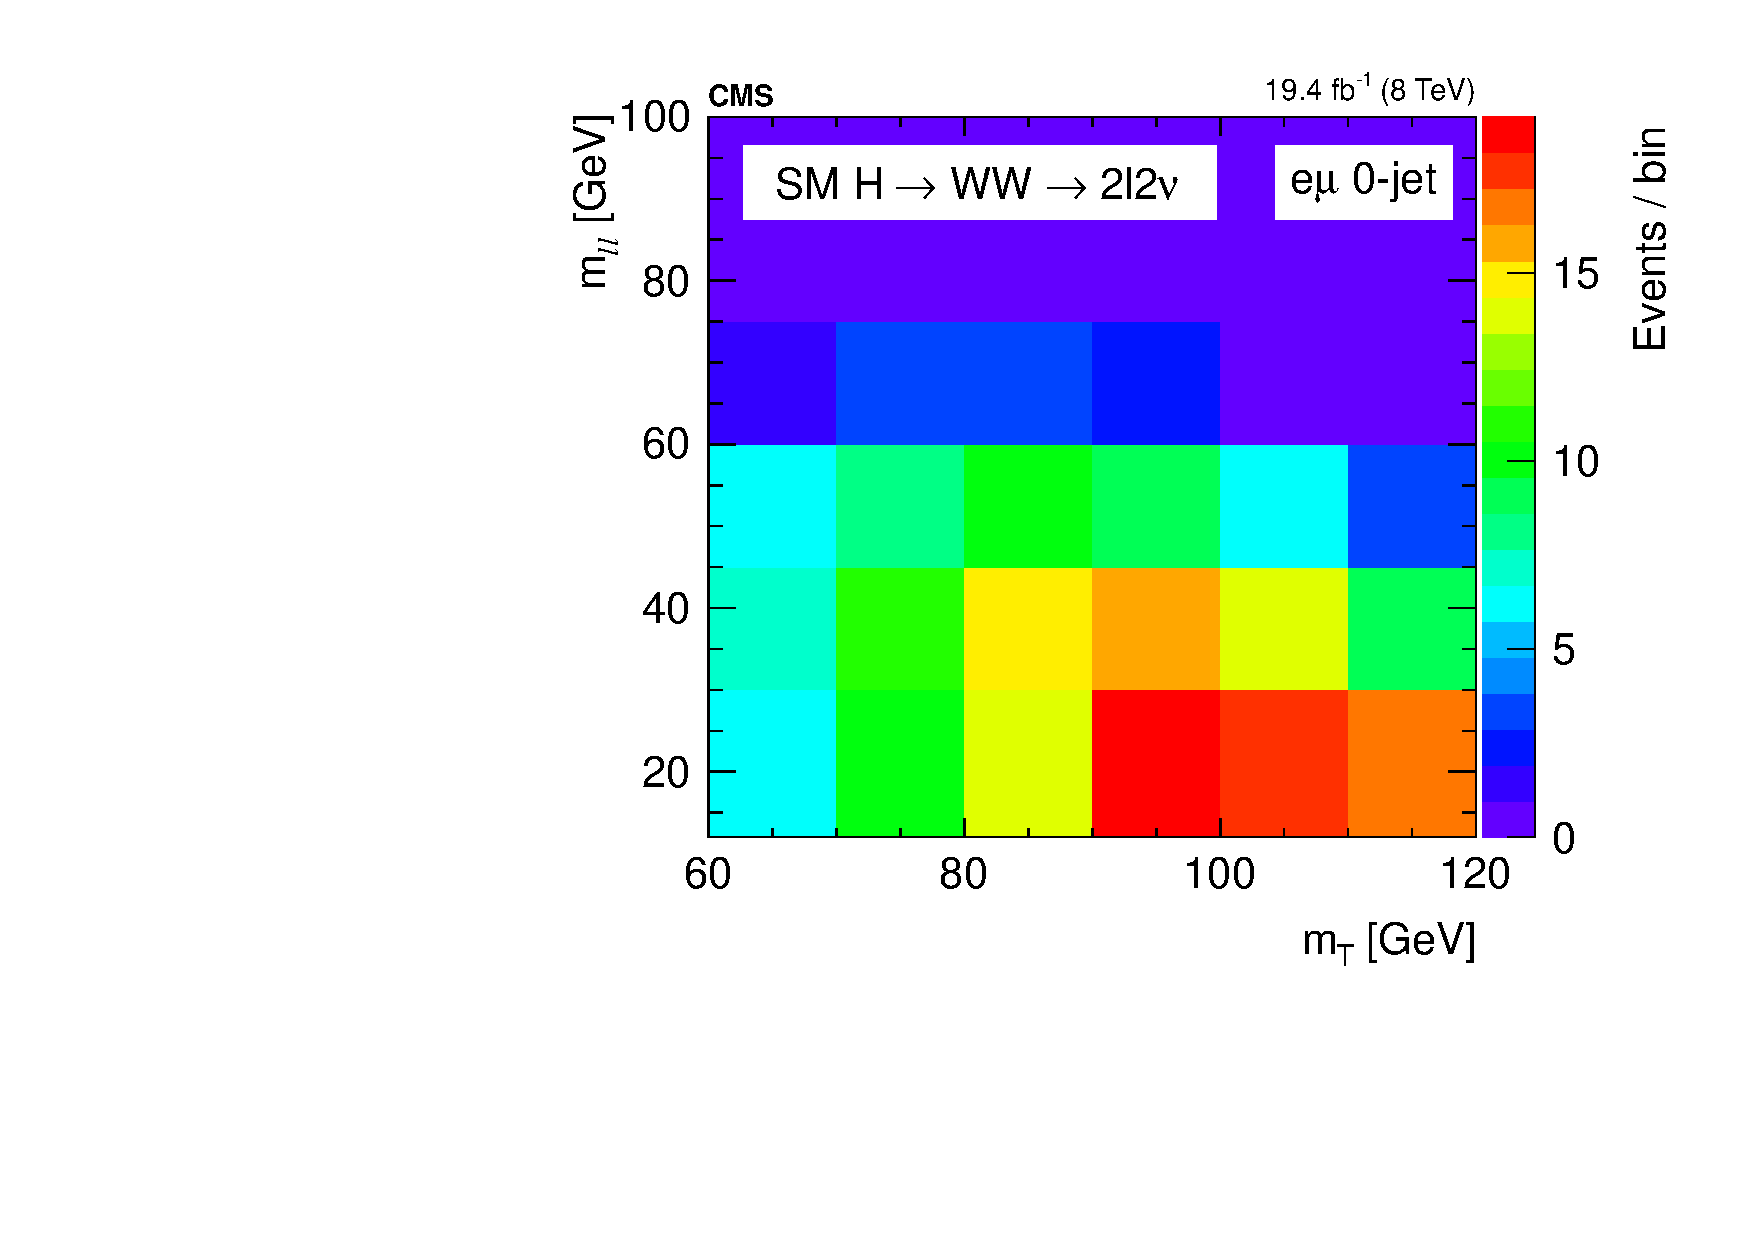
\includegraphics[width=0.45\textwidth]{figures/2d_prefit_0j_125_sig_paper.pdf}
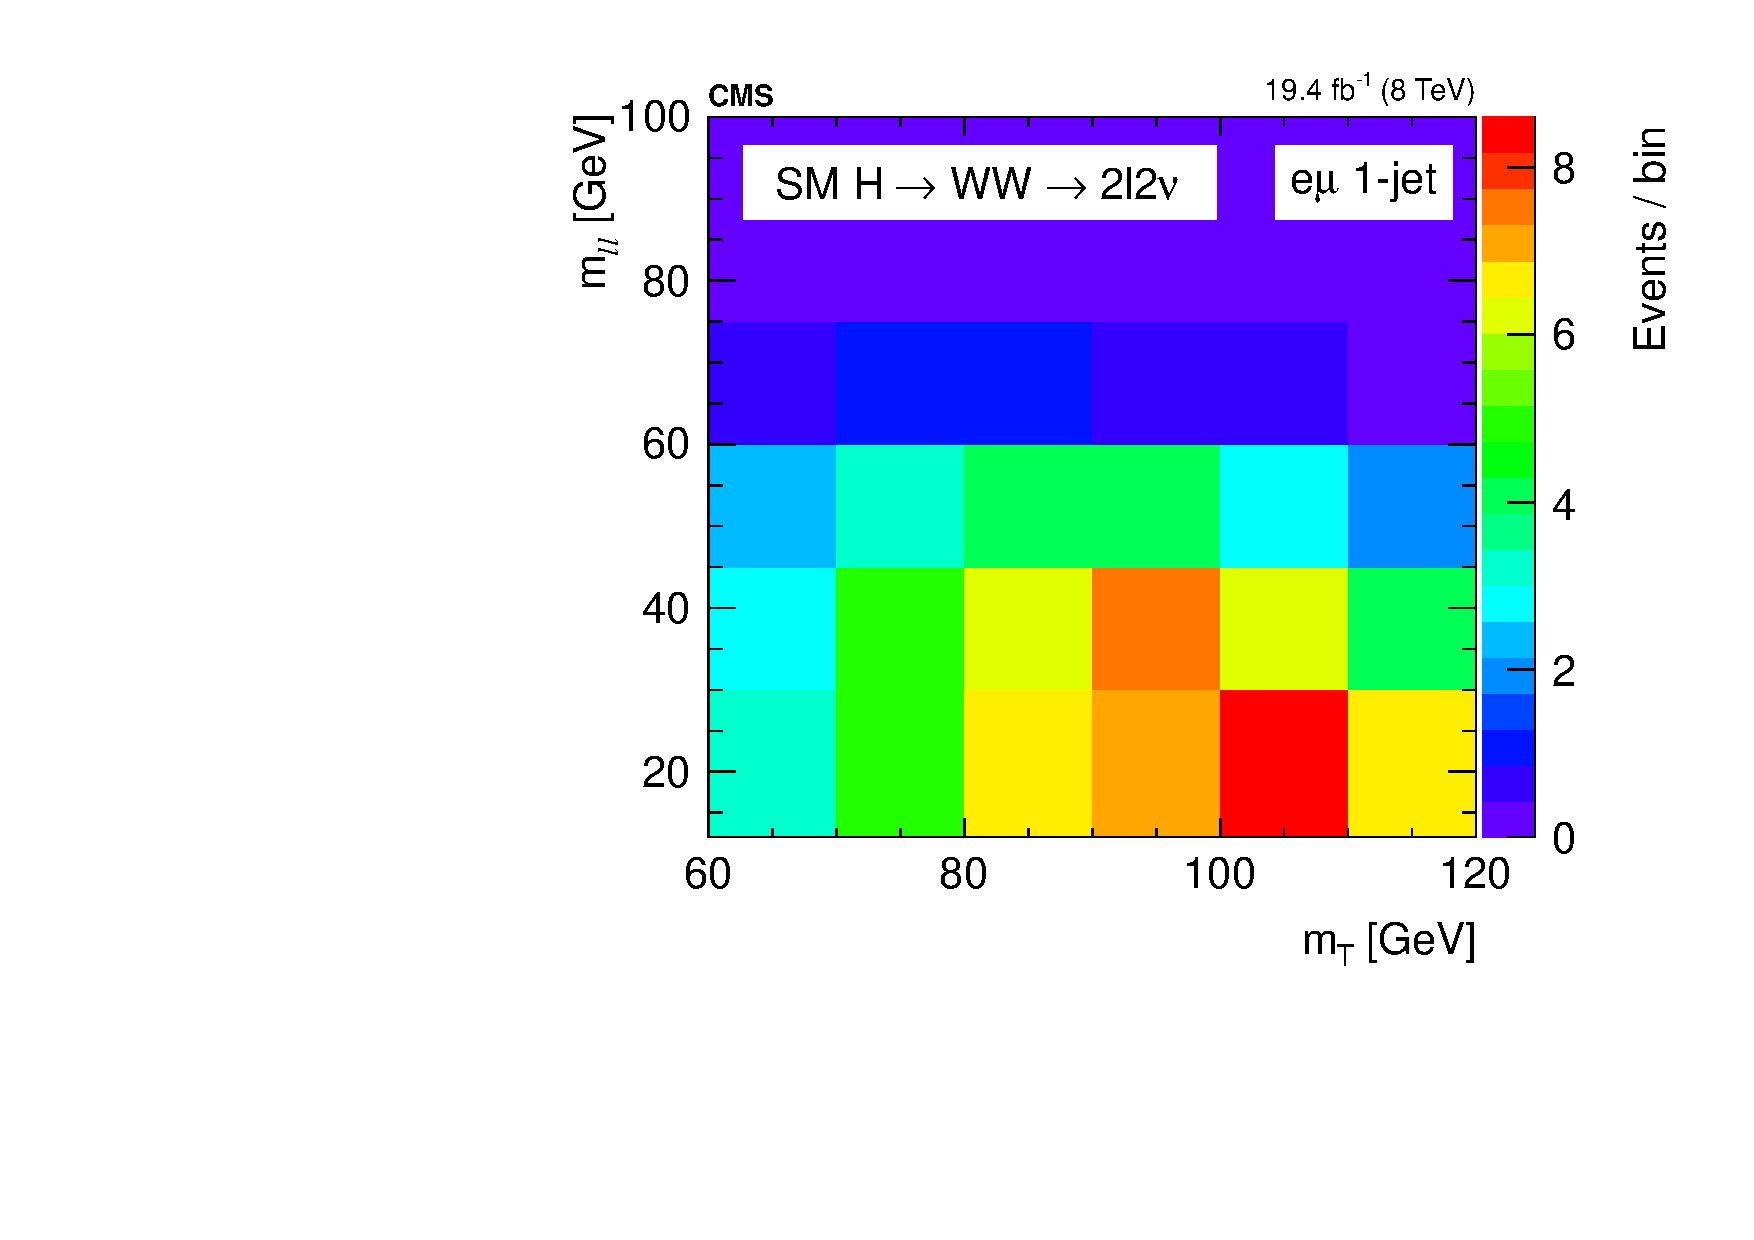
\includegraphics[width=0.45\textwidth]{figures/2d_prefit_1j_125_sig_paper.pdf}
\\
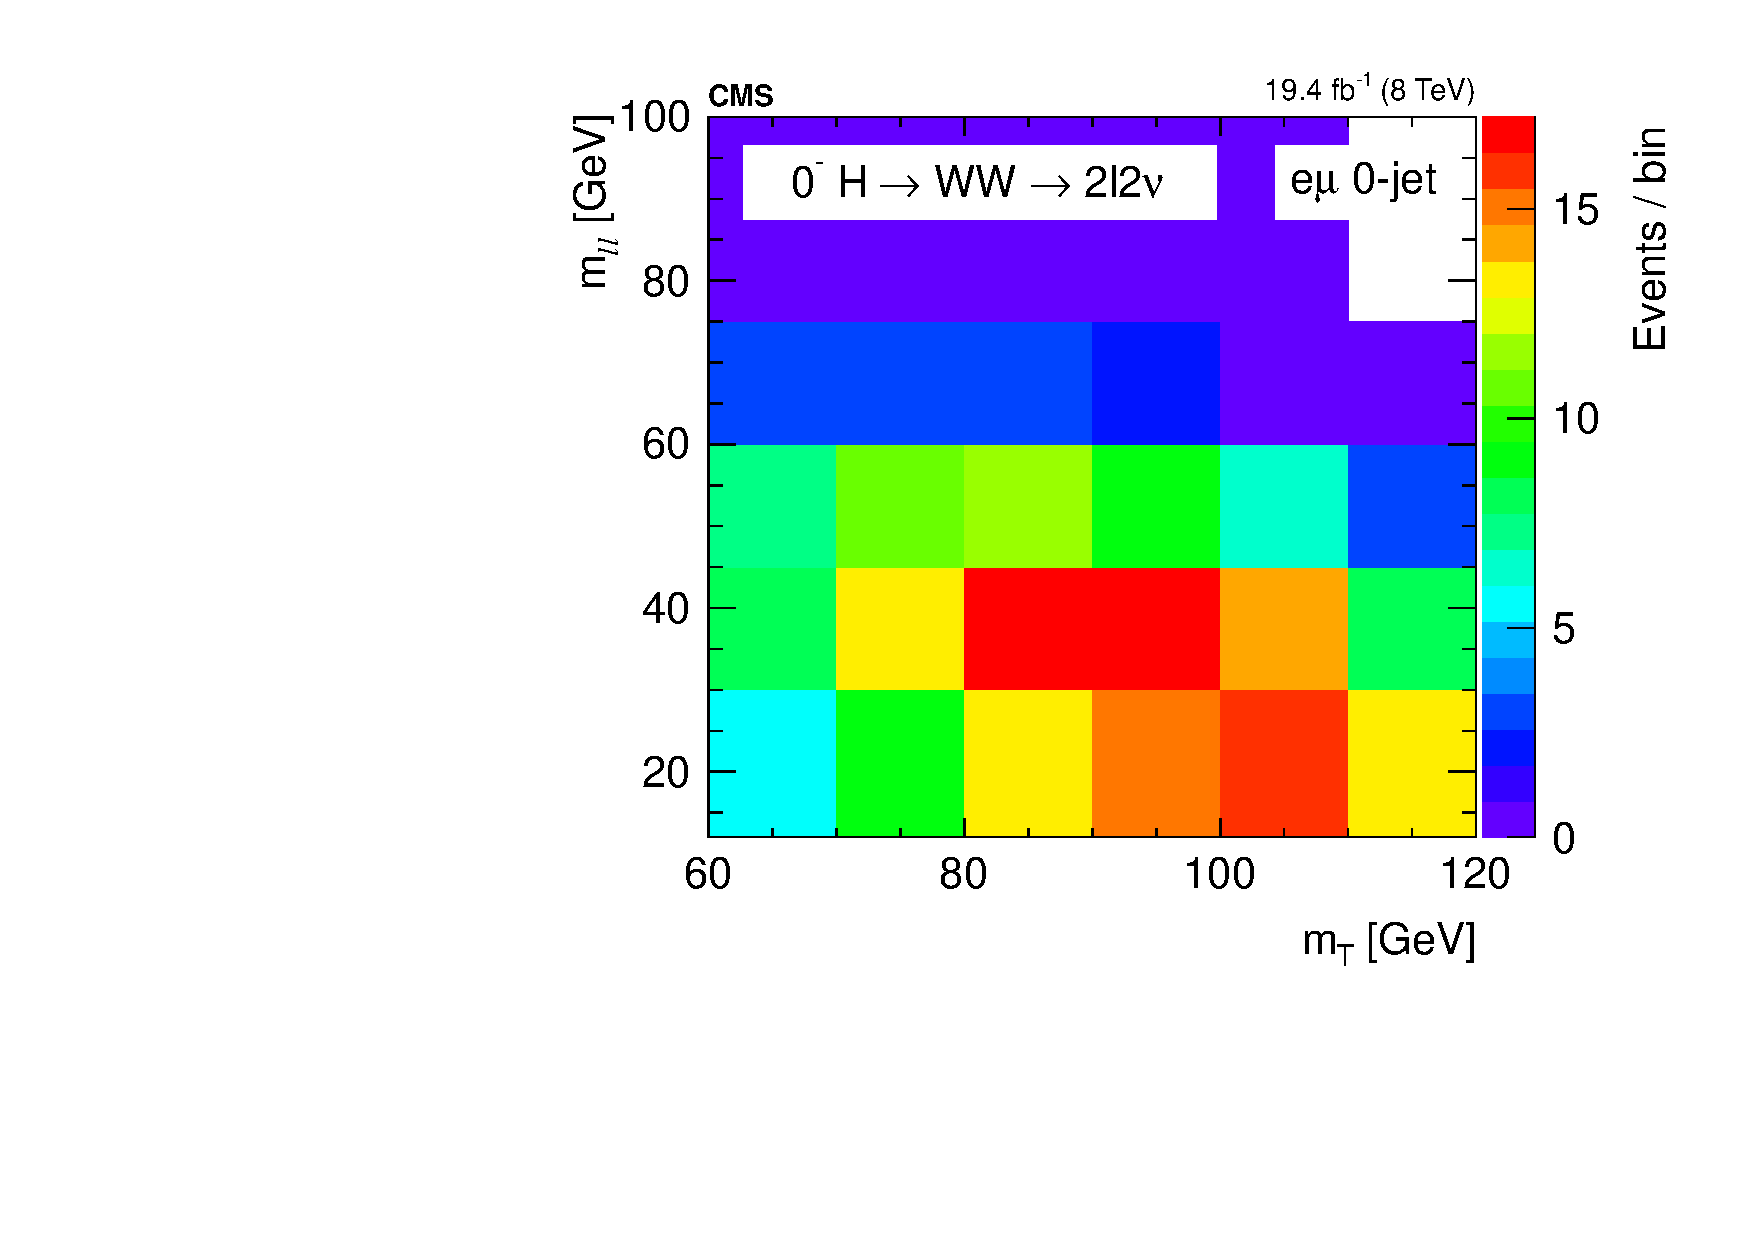
\includegraphics[width=0.45\textwidth]{figures/2d_prefit_0j_125_spin0m_paper.pdf}
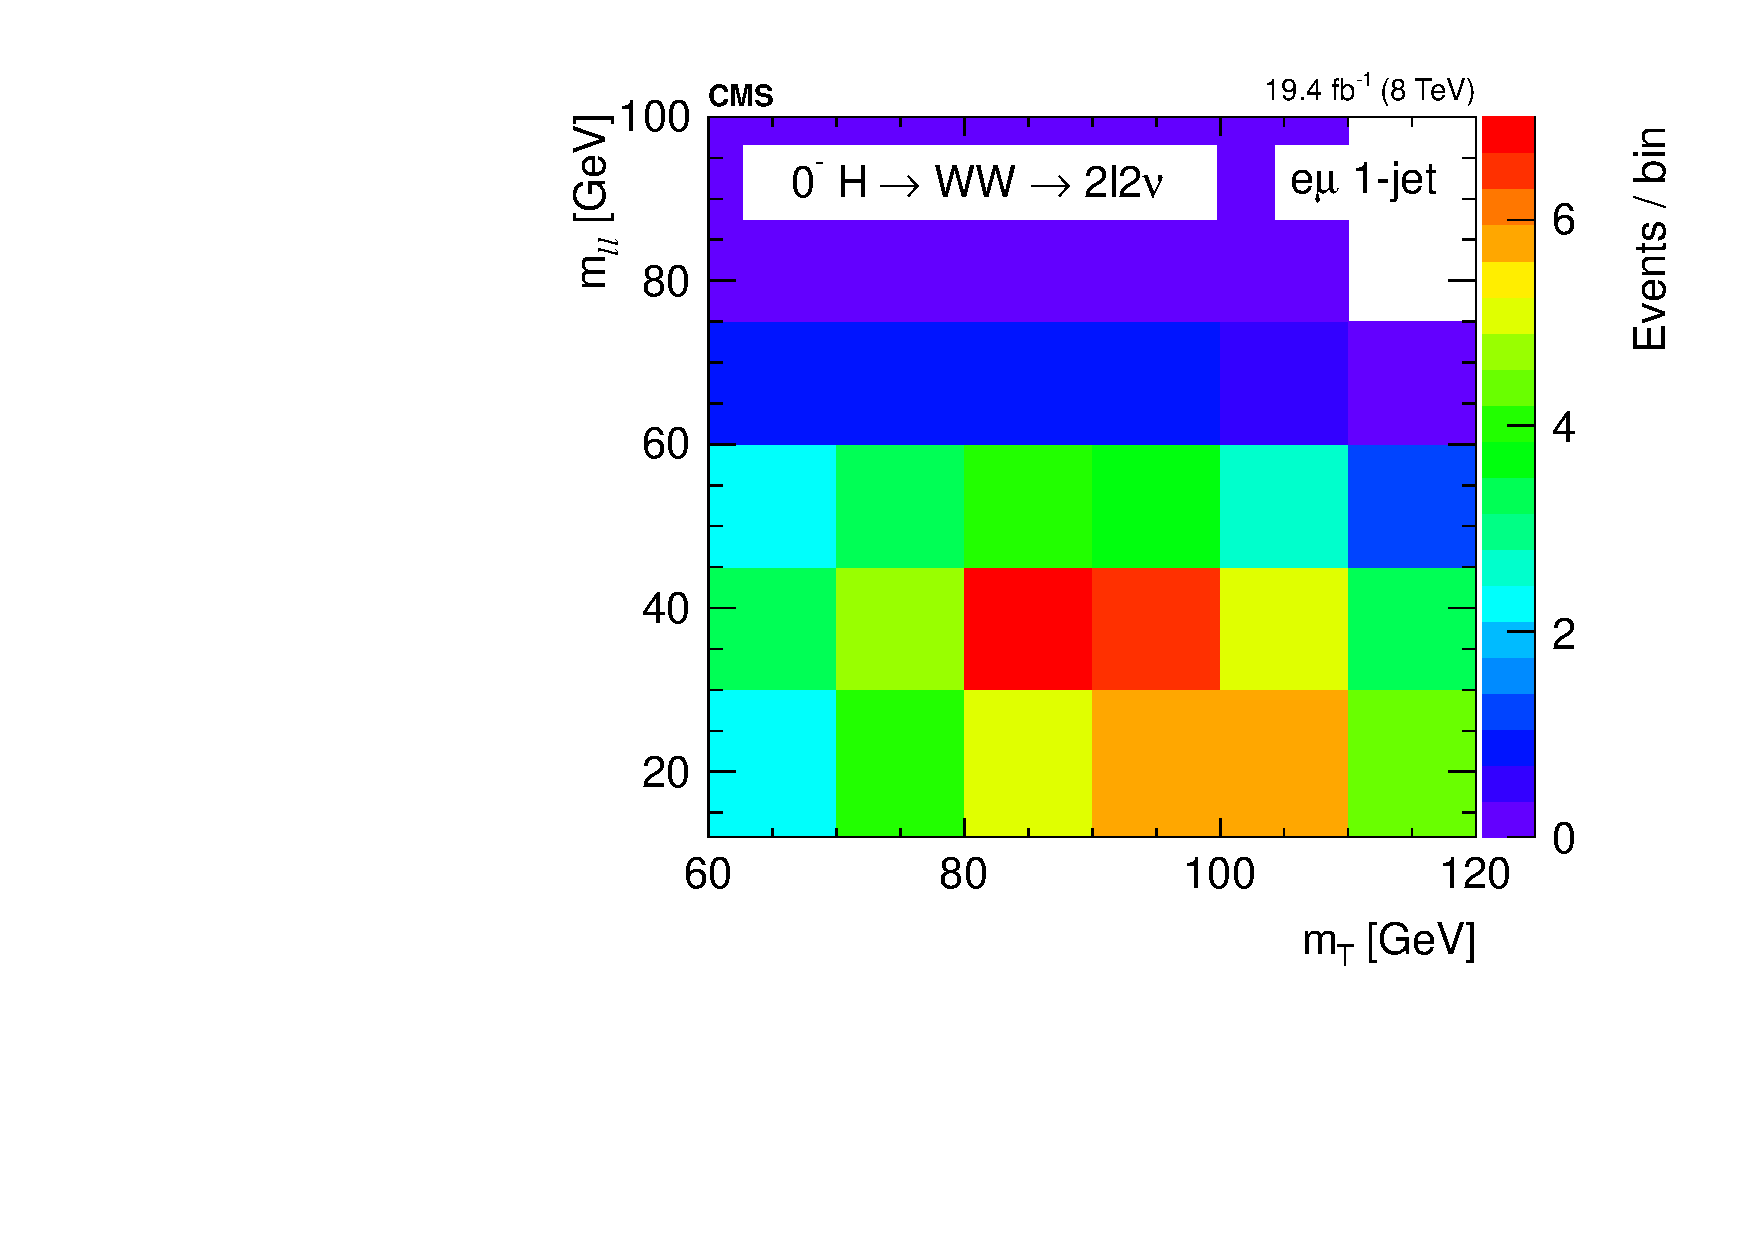
\includegraphics[width=0.45\textwidth]{figures/2d_prefit_1j_125_spin0m_paper.pdf}
\\
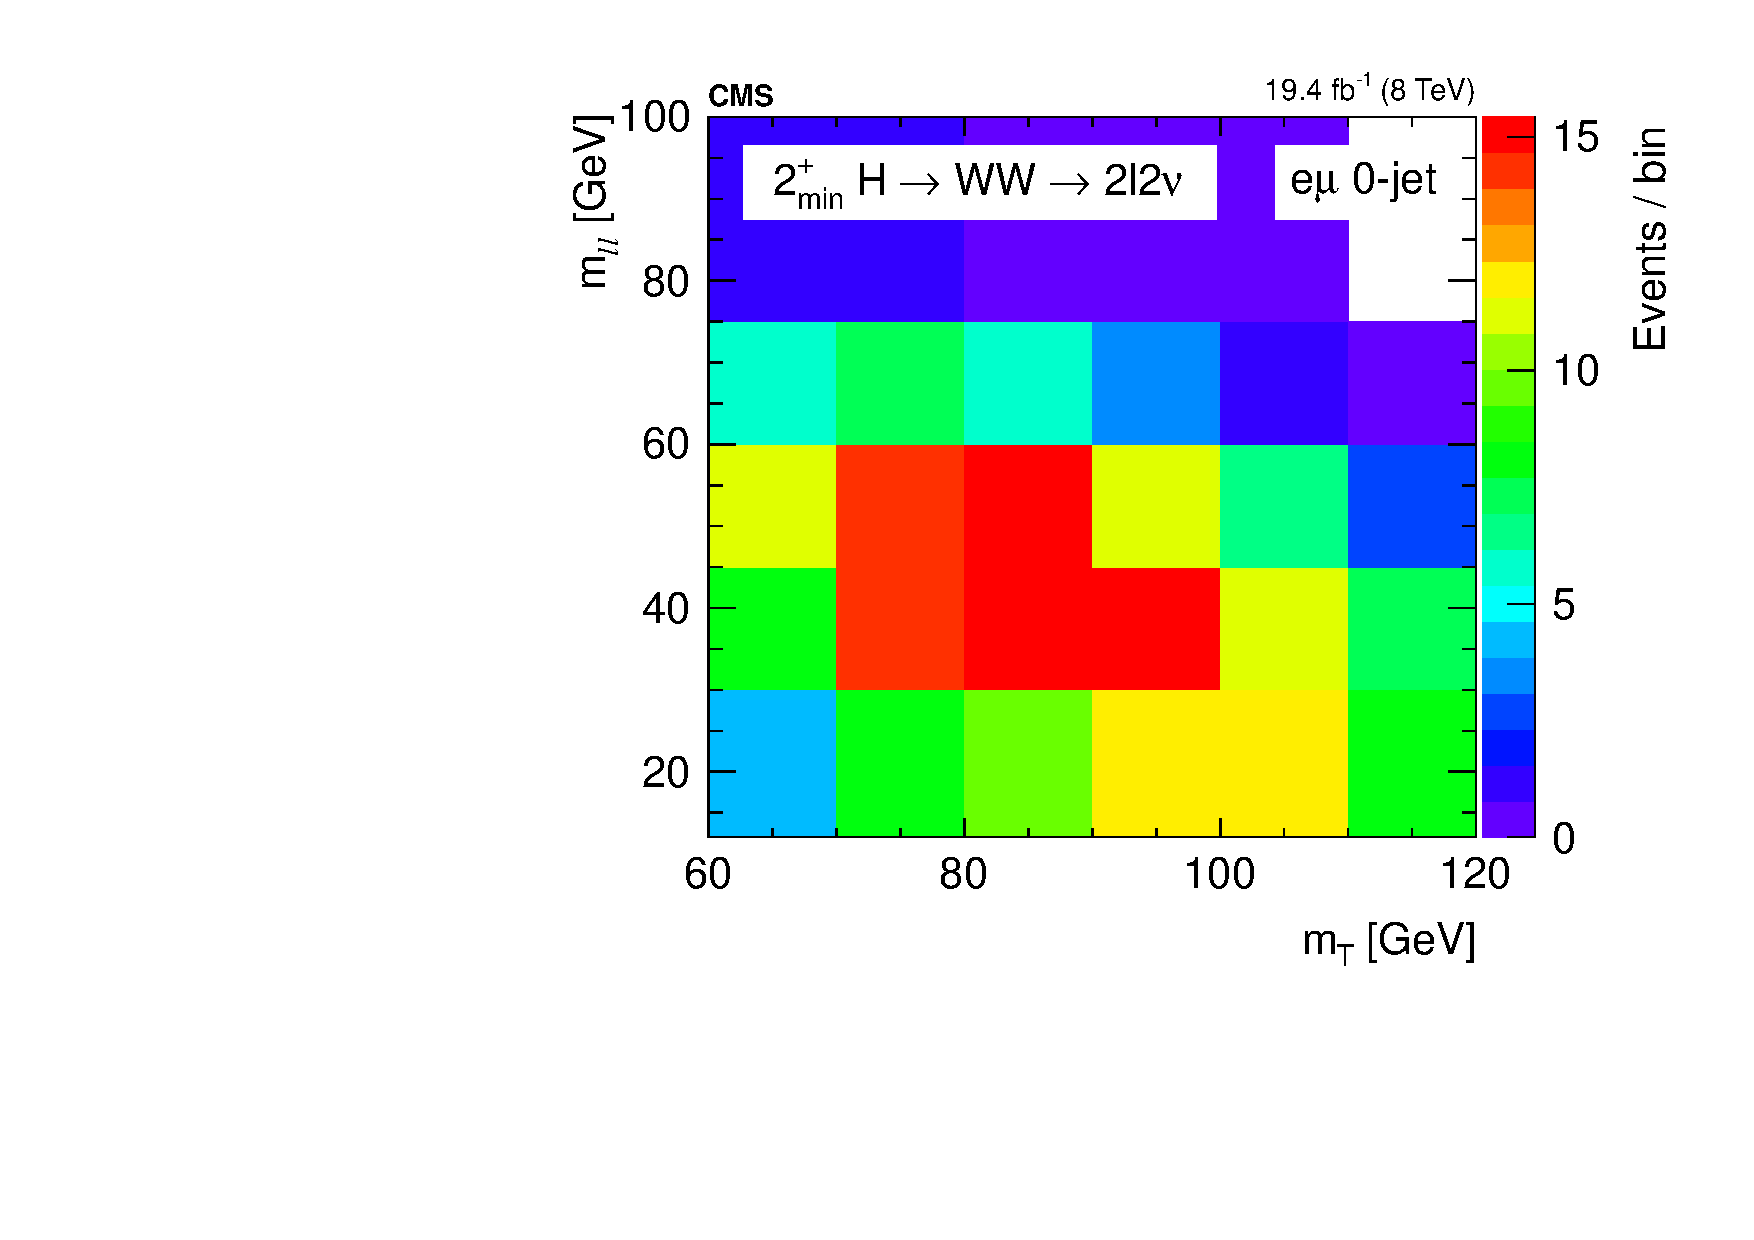
\includegraphics[width=0.45\textwidth]{figures/2d_prefit_0j_125_spin2_paper.pdf}
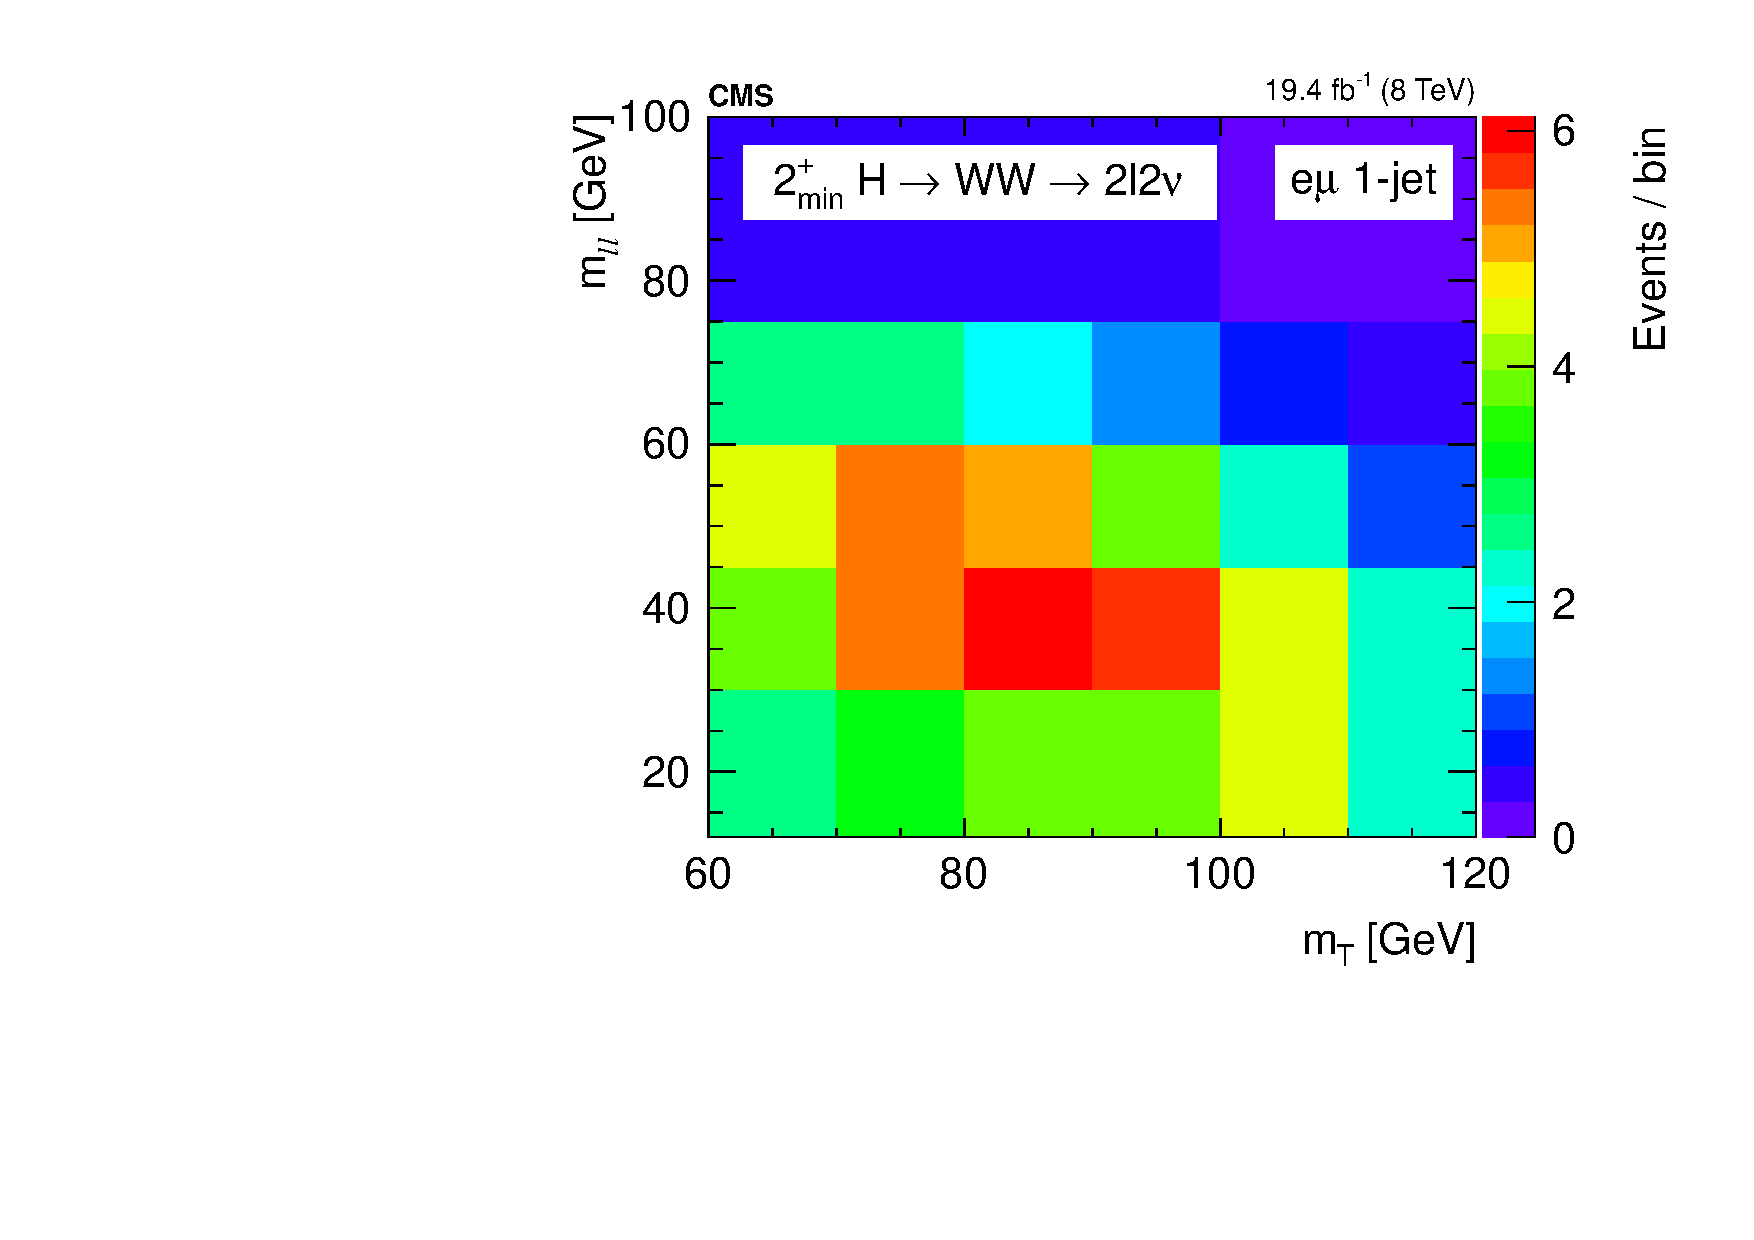
\includegraphics[width=0.45\textwidth]{figures/2d_prefit_1j_125_spin2_paper.pdf}
\caption{2-dimensional templates for $0^+$, $0^-$ and $2_{min}^+$ models.} 
\label{fig:2dtemplates_spin} 
\end{figure} 

Figure~\ref{fig:2dtemplates_spin} shows the 2-dimensional templates zoomed in the signal region
($60<\mT<120~\GeV$ and $0<\mll<100~\GeV$) for SM Higgs boson($0^+$), 
pseudo-scalar boson($0^-$) and the $2_{min}^+$ model in 0-jet and 1-jet categories. 
In both categories it is clearly seen that the $2_{min}^+$ and $0^+$ hypotheses have different shapes,
and this information can be used to discriminate one from the other.
On the other hand, the difference between $0^+$ and $0^-$ 
is not seen as much as the $2_{min}^+$ case. 
Thus, the separation between $0^+$ and $0^-$ model is not expected to be 
as strong as the $2_{min}^+$ case.  
For the backgrounds, the exactly same templates are used as in the 
search analysis. They are shown in Figure~\ref{fig:2dtemplate_125_0j_1}
- \ref{fig:2dtemplate_125_0j_4} for 0-jet. 
%\textcolor{red}{what about 1-jet templates?} 

\subsubsection{Test statistic}

For the statistical interpretation, we construct the test statistic($q$). 
It is defined as the difference of the log likelihood between the two 
hypotheses, \textit{i.e.}, alternate model($J^P$) vs. SM Higgs boson($0^+$), 
\begin{eqnarray} 
q_{J^P} = -2 \ln \mathcal{L}_{J^P} / \mathcal{L}_{0^+}  
\end{eqnarray} 
The likelihood is same as the one used in the SM Higgs search :  
\begin{eqnarray} 
\mathcal{L} ( X | \mu, \theta) 
\, = \,
\prod_{i}^{N_{bin}} \frac{ \left( \mu s_i(\theta) + b_i(\theta) \right)^{X_i}}{X_i!} 
\, e^{ - \mu s_i(\theta) - b_i(\theta) }   \times
\prod_{j}^{N_{nuisance}} p\left( \tilde{\theta_j} | \theta_j \right).
\end{eqnarray}
The only difference in the two likelihoods is the signal component, $s_i$.

We perform a maximum likelihood fit for each hypothesis with the same dataset,
and the difference in the log-likelihood is taken as a test statistic. 
In the two fits, the signal strength is allowed to float independently, 
and the nuisance parameters in the two models are treated independently. 
The $q_{J^P}$ is calculated using the best-fit values of the nuisance parameters. 

\subsubsection{Quantifying the separation}

The separation is quantified by measuring imcompatility of data with 
the hypothesis under consideration. The expected separation is defined as  
\begin{eqnarray} 
P(q > q_{0^+}^{\textrm{expected}} | \textrm{ alternate model}) 
\end{eqnarray} 
where $q_{0^+}^{\textrm{expected}}$ is the peak position of $q$ assuming $0^+$.
For the observed separation, we can use the observed $q$ from data. 

%%%%%
\section{Results}

Because the $2_{min}^+$ model can be generated via both $gg\rightarrow X$ 
and $q\bar{q }\rightarrow X$ modes, and the result depends on the fraction of the two modes, 
the results is reported as a function of the fraction of the $q\bar{q} \rightarrow X$ production mode, 
$f_{q\bar{q}}$. The $0^-$ model is generated via only $gg\rightarrow X$,
so only one result is reported. The alternate models are normalized to the 
SM Higgs cross section. The \qqH\ and \qqVH\ modes are not tested in this study, 
\textit{i.e.} the SM Higgs prediction is used for both hypotheses. 

Figure~\ref{fig:llr_spin2} shows the distribution of $q_{2_{min}^+}$ with full data 
combining 0-jet and 1-jet categories. 
Figure~\ref{fig:llr_band} shows the expected median, $\pm1\sigma$(green) 
and  $\pm2\sigma$(yellow) bands for $q$ assuming $0^+$. 
When the observed $\mu$ is used, the expected separation ranges from 
$1.8\sigma$ to $2.9\sigma$ as $f_{q\bar{q}}$ goes from 0 to 100~\%.
The incompatibility of data with $2_{min}^+$ model ranges from  
$1.2\sigma$ to $3.1\sigma$ as $f_{q\bar{q}}$ goes from 0 to 100~\%.
We can express this result in terms of \CLs. The \CLs\ ranges from 
16.3~\% to 0.2~\% as $f_{q\bar{q}}$ goes from 0 to 100~\%.
All these result shows that data prefers $0^+$ to $2_{min}^+$ hypothesis.  

Figure~\ref{fig:llr_spin0m} shows the distribution of $q_{0^-}$ with full data 
combining 0-jet and 1-jet categories. When the observed $\mu$ is used, 
The expected separation is $0.8\sigma$.  
As expected in the 2-dimensional templates in Figure~\ref{fig:2dtemplates_spin},
the sensitivity of separation between $0^+$ and $0^-$ is 
not as good as the $2_{min}^+$ case.
The observed separation is $1.2\sigma$, and it corresponds to \CLs=34.7~\%. 

%
\begin{figure}[ht!] 
\centering 
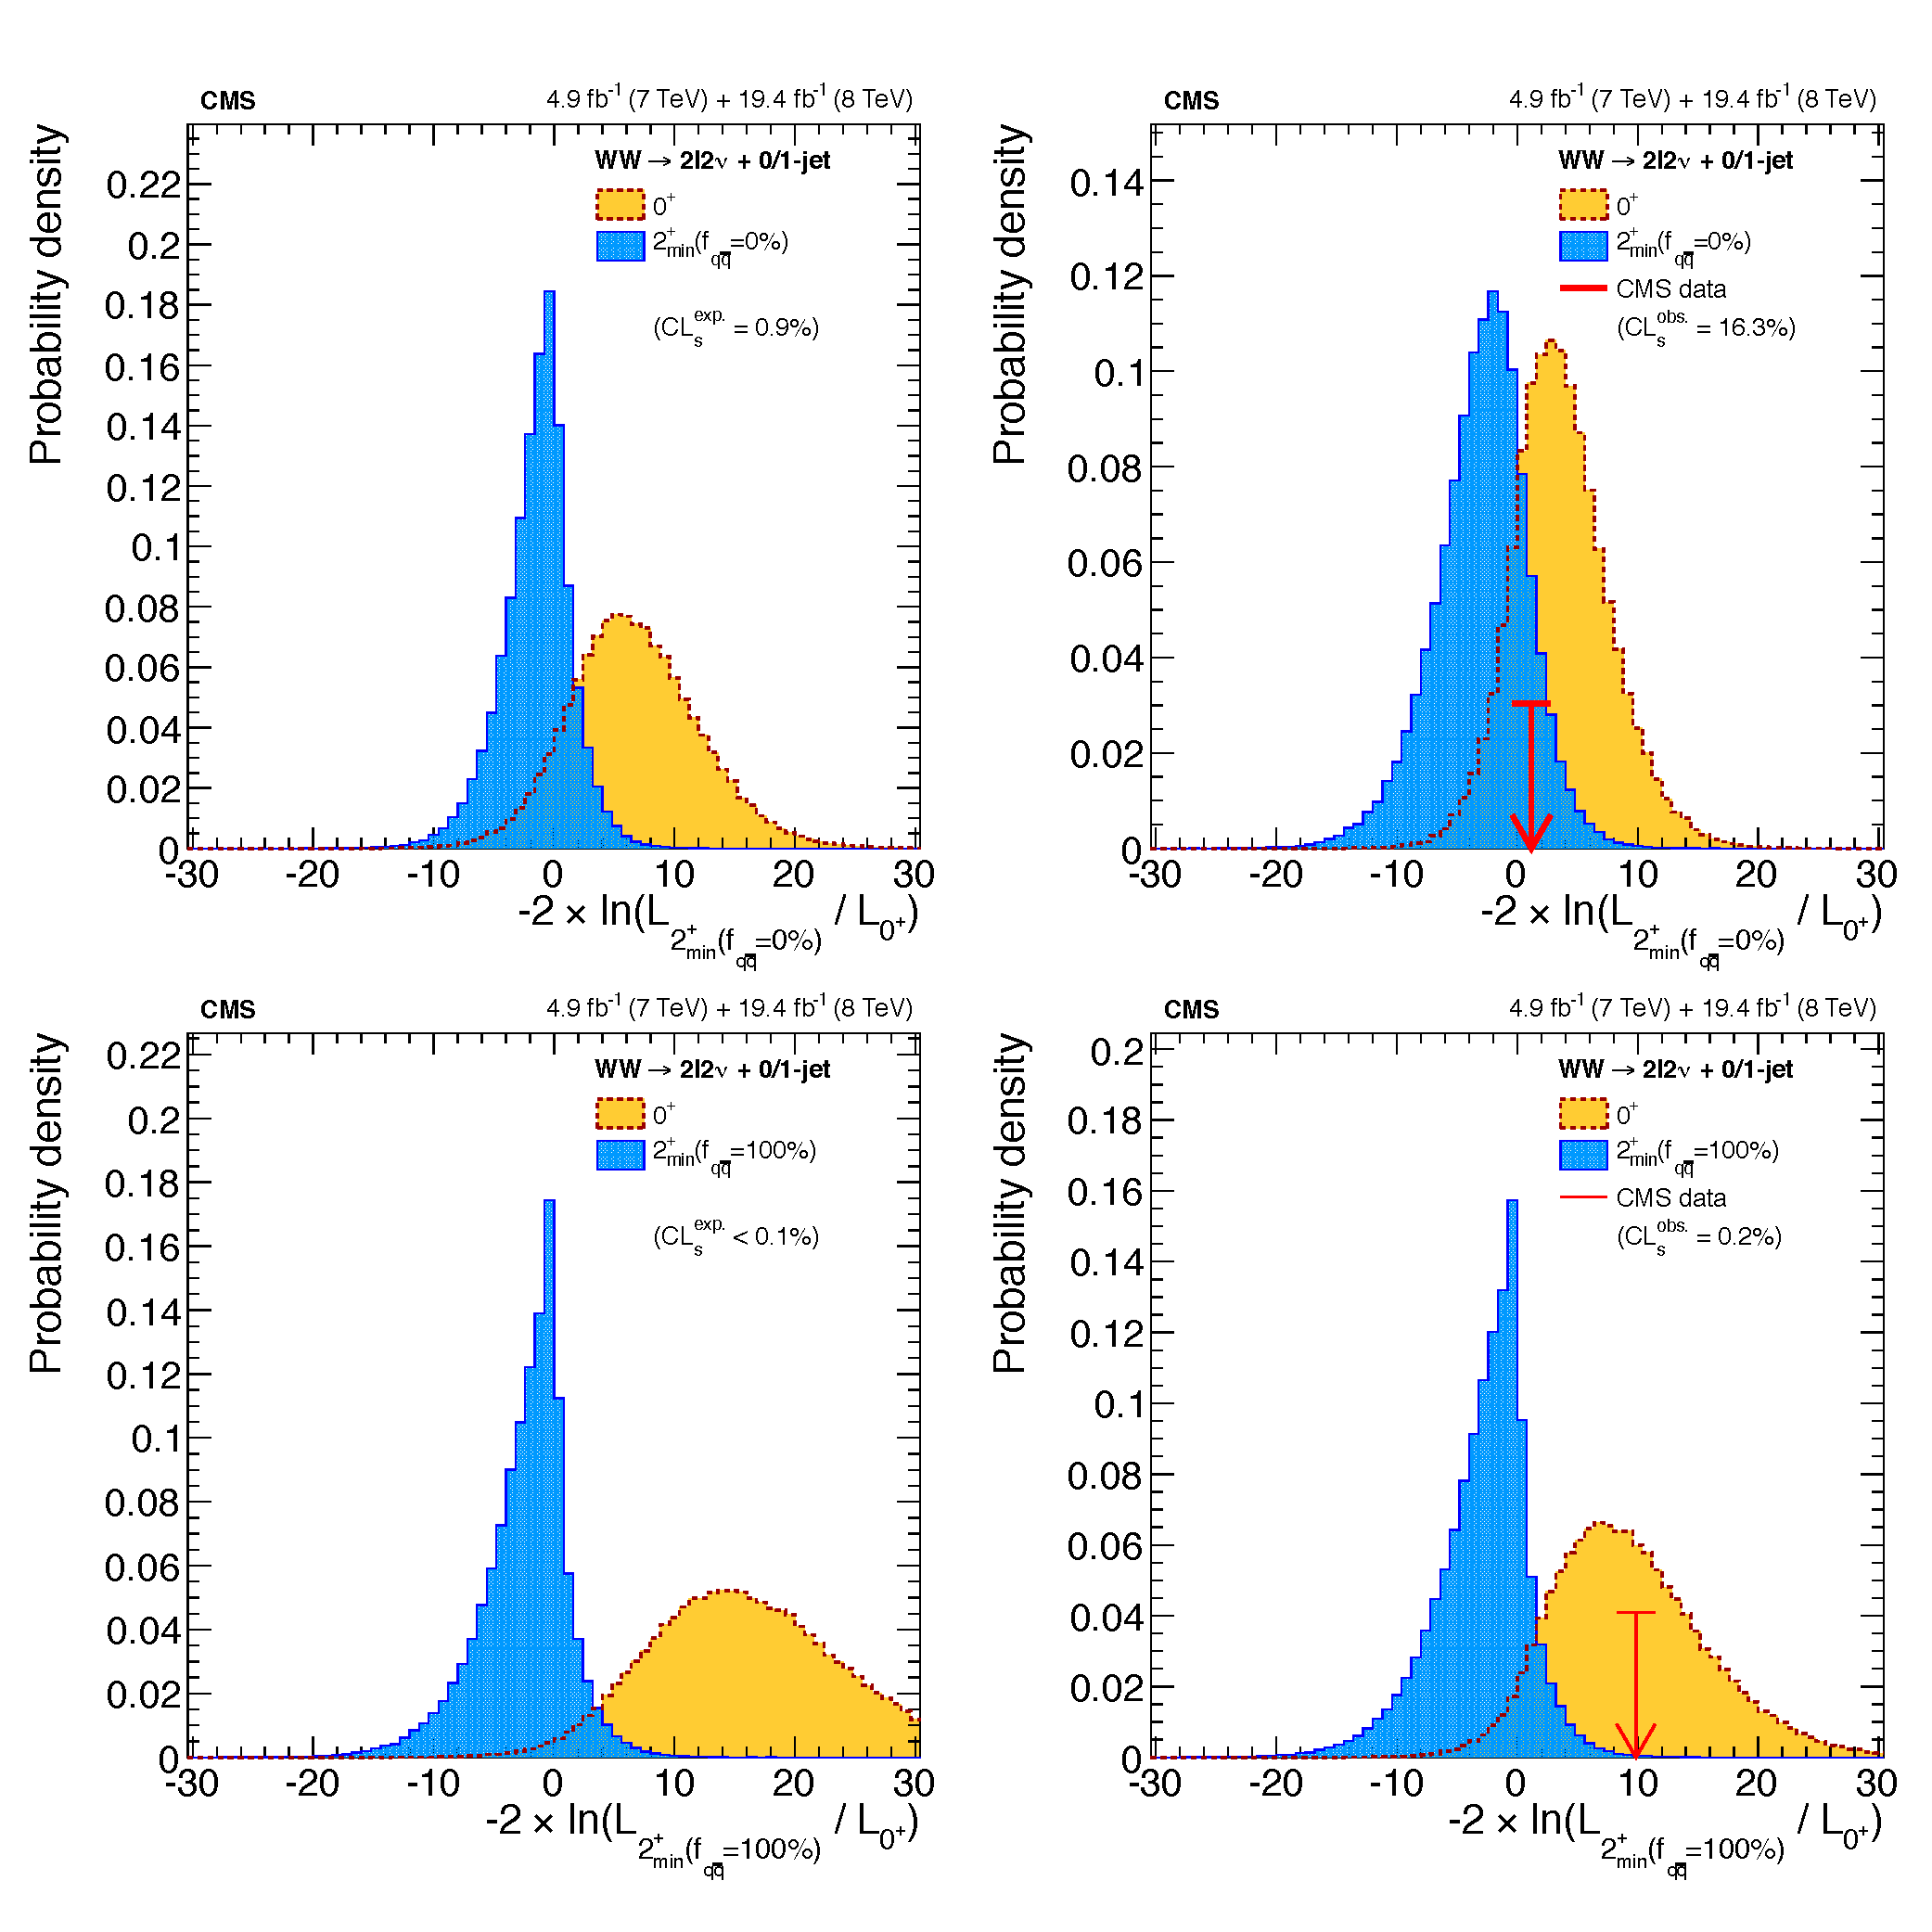
\includegraphics[width=0.9\textwidth]{figures/spin2LLR.pdf}
\caption{Distributions of $q_{2_{min}^+}$ assuming $0^+$ and $2_{min}^+$ models.  
The blue is the expected distribution assuming 
$2_{min}^+$, and the orange is the expected distribution assuming $0^+$ hypothesis.
Top plots show the result with $f_{q\bar{q}}=0~\%$ and the bottom plots show 
the result with $f_{q\bar{q}}=100~\%$. The left plots show the result using the 
expected signal signal strength, $\mu=1$, 
and the right plots show the result using the best-fit value of the signal strength, 
$\mu \approx 0.75$.}  
\label{fig:llr_spin2} 
\end{figure} 
%
\begin{figure}[ht!] 
\centering 
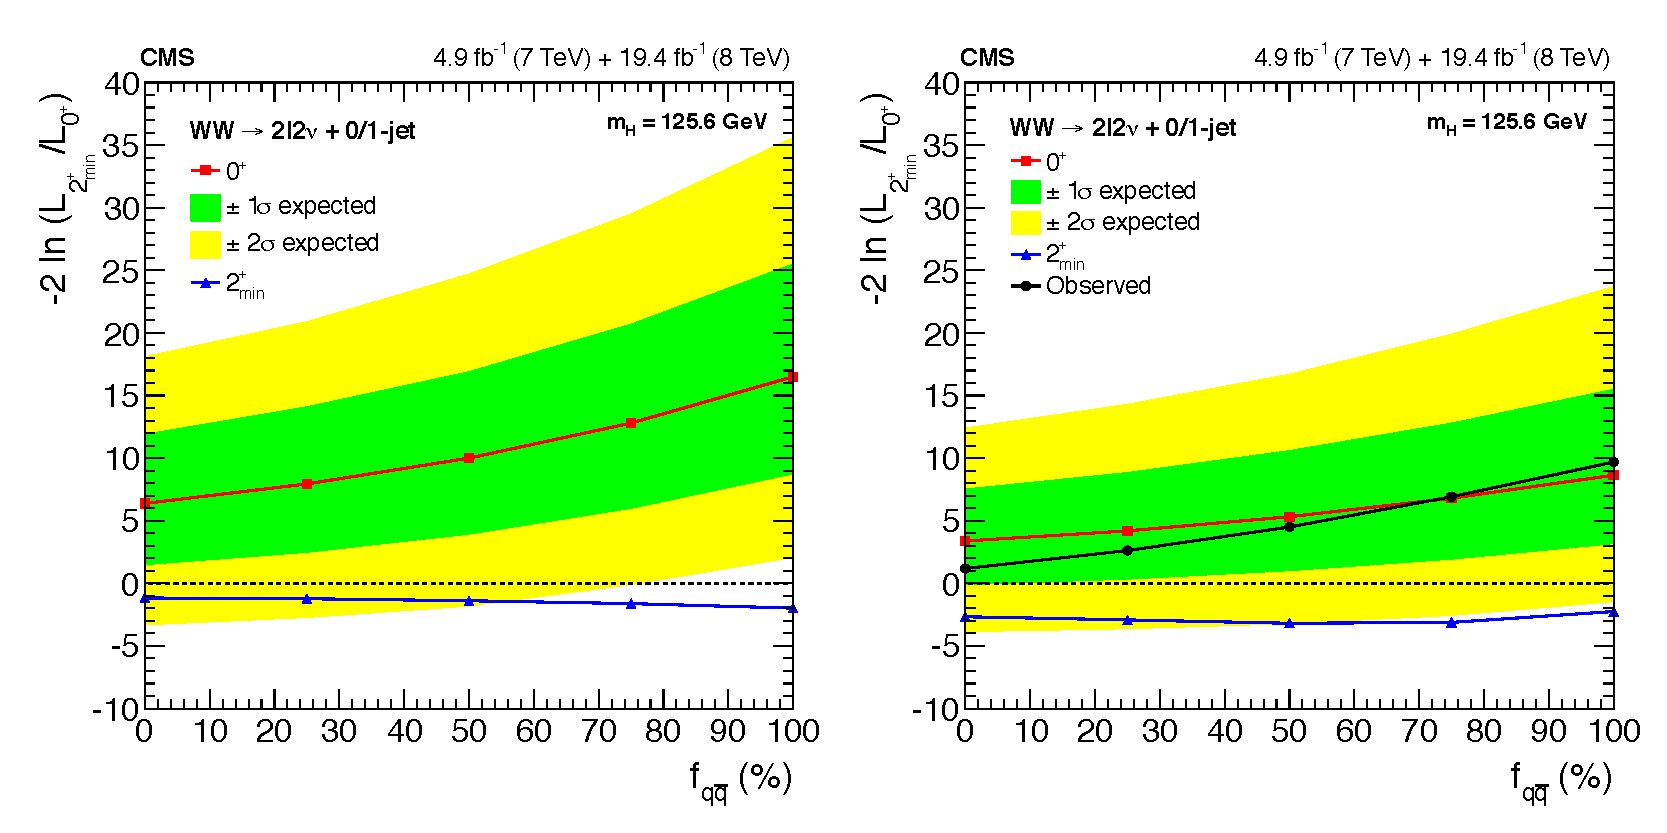
\includegraphics[width=0.9\textwidth]{figures/spinLLRband.pdf}
\caption{Median of $q_{2_{min}^+}$ as a function of $f_{q\bar{q}}$. 
The blue line is the median of $q$ assuming $2_{min}^+$.
Left is with $\mu=1$ and the right is with observed $\mu$.
Right plot also shows the $q$ calculated using data. 
} 
\label{fig:llr_band} 
\end{figure} 
%
\begin{figure}[ht!] 
\centering 
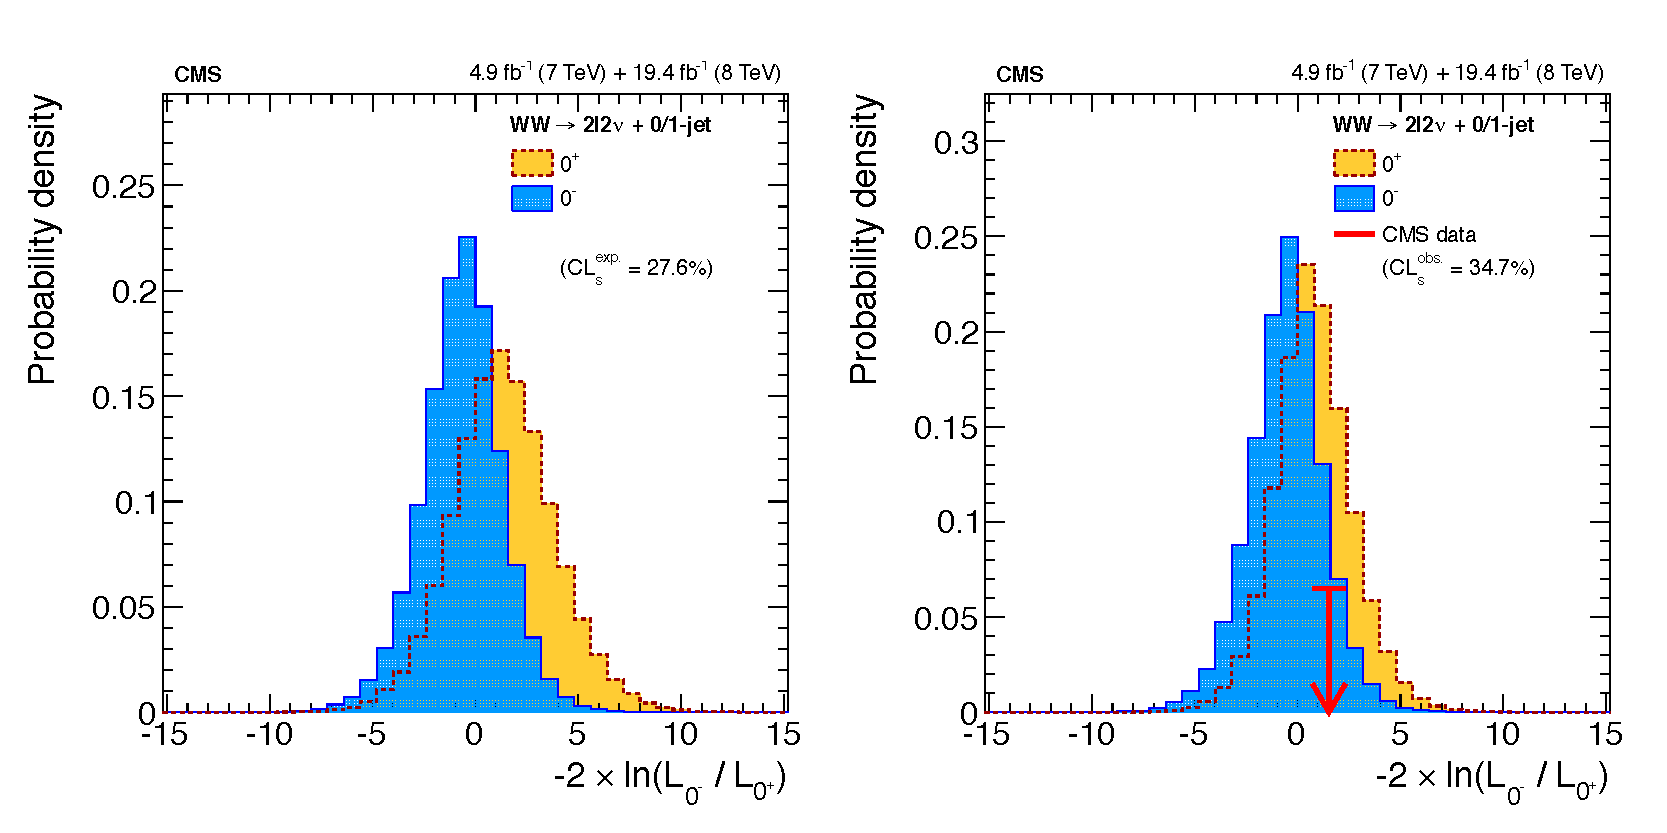
\includegraphics[width=0.9\textwidth]{figures/spin0mLLR.pdf}
\caption{Distributions of $q_{0^-}$ assuming $0^+$ and $0^-$ models.  
Blue is the expected distribution assuming $0^-$, 
and orange is the expected distribution assuming $0^+$ hypothesis.
The left plots show the result using the expected signal signal strength, $\mu=1$, 
and the right plots show the result using the best-fit value of the signal strength, 
$\mu \approx 0.75$.}  
\label{fig:llr_spin0m} 
\end{figure} 

%%%%%%%%
\section{Conclusion of spin-parity study} 

A test on the spin-parity nature of the new boson is performed against two alternate 
models, $2_{min}^+$ and $0^-$. The result shows that data favors $0^+$ to 
$2_{min}^+$ with \CLs=0.2-16.3~\% depending on the fraction of 
$q\bar{q}\rightarrow X$ mode. The \CLs\ with $0^-$ model is 34.7 \%.  


